\section{Introduction\label{sec:ch4:introduction}}

Dynamics play an increasingly important role in the advancement of many complex engineering systems \cite{Allison2014a}.
The primary goal of design studies is to find solutions and gain a general understanding of the design trade-offs, building design knowledge for the particular system.
Here we show how scaling can facilitate finding accurate, generalizable, and intuitive information for the design problem at hand.

% new paragraph
At a basic level, scaling is simply the stretching, squeezing, and shifting of the problem elements and this can include the time continuum, design variables, constraints, objective function, etc.
For example, if we have the inequality constraint $a x \leq b$ and $b > 0$, then we can arrive at an equivalent scaled constraint $\rho x \leq 1$ where $\rho=a/b$.
The mechanics of scaling are fairly straightforward but proper utilization of scaling is heavily reliant on the creativity and intuition of the designer \cite{Holmes2009a}. 
This barrier may be one of the reasons why scaling is often overlooked, but these manipulations can help define problem formulations that are 1) better suited for analysis and 2) more favorable for solution methods (e.g.,~higher quality solutions and faster convergence). 
In this chapter, we provide the necessary theory to scale \glsfoo[noindex]{DO} problems and some examples of how to use scaling in the context of a design study.

% new paragraph
First, we review some of the previous uses of scaling focusing on examples relevant to obtaining solutions and the analysis of engineering design problems.
Some of these examples are quite well-established, while others are rarely used. 
The context that all the examples provide is crucial for defining the most useful scaling procedure for a particular design problem.
Some authors state that the importance of scaling can only be fully appreciated through examples \cite{Groesen2007a}.

\subsection{Previous Uses of Scaling \label{sec:ch4:uses}}

% new paragraph
One of the primary uses of scaling is to reduce the number of parameters in a set of equations \cite{Cengel2006a, Groesen2007a,Holmes2009a}.
Under certain conditions, algebraic manipulations can lead to a reduced set of parameters (e.g.,~consider the example above where now $\rho$ is the only parameter).
Buckingham's Pi theorem is one well-known method for reducing the number of parameters, which applies constraints on the mathematical interaction of the fundamental units of the system and does not necessarily need a specific mathematical expression of the system (e.g.,~the equations of motion) \cite{Buckingham1914a, Holmes2009a, Groesen2007a}.
However, this approach does not necessarily leverage the equations of motion nor does it directly consider the numerical aspects of finding approximate solutions to the system of equations. 

% new paragraph
Another common use for scaling is to determine characteristic properties of the system. These properties may be scalars or functions. Characteristic scalars are well studied in many engineering domains such as fluid dynamics and heat transfer \cite{Cengel2006a}. An example of such a scalar is the Reynolds number, a dimensionless constant that relates inertial forces to viscous forces within a fluid \cite{Cengel2006a}. Other examples include intrinsic resonance frequency, length, damping, or time constant.  Such characteristic properties can be conceptually easier to understand \cite{Holmes2009a}.
These properties may be well understood for classical domains but for others, these characteristic properties may be the key to building the required knowledge of the system.

% new paragraph
In dynamic or spatially-defined systems, it can be advantageous to scale entire continuous functions. For example, for an initial value problem, characteristic solutions to the differential equation can be obtained that scale linearly with the initial condition \cite{Holmes2009a}. Under certain conditions, even the solution to optimization problems can be scaled for different parameter values. There are some potentially restrictive issues with directly scaling optimal solutions that are discussed in Ref.~\cite{Kittirungsi2008a}. 

% new paragraph
The central tool in many design studies is design optimization.
Frequently, the solution of a single optimization problem is not sufficient to address the complicated nature of a design activity.
This typically leads to variations on the problem formulation elements (e.g.,~parametric sweeps of the problem's parameters).
Both reducing the number of parameters and obtaining scalable solutions can greatly improve this process.

% new paragraph
Scaling can also be used to help decide if certain parts of a model or optimization formulation are small, and therefore negligible in a consistent manner \cite{Holmes2009a, Khalil2002a}.
This can help with developing asymptotic solutions to differential equations, reveal multiple-time-scale structures, and simplify simulations, stability analysis, and controller design \cite{Khalil2002a}.
With respect to optimization formulations, scaled forms of the constraints can help determine if certain constraints are likely to be active or inactive based on the magnitude of their scaled forms \cite{Papalambros2017a}.

% new paragraph
One common motivation for scaling in optimization is to change the order of magnitude of the variables and constraints to be more favorable for computation \cite{Papalambros2017a, Rao2010a}.
Large order of magnitude differences in either the variables or function values can produce ill-conditioned matrices such as Jacobians and Hessians; thus, algorithmic calculations may become unstable or inefficient \cite{Papalambros2017a}.
Systematic preconditioning methods have been developed to scale special cases of problem elements such as linear constraints \cite{Bergamaschi2004a, Benzi2002a}.
This has been observed to be especially important in DO to ensure robustness and accuracy \cite{Rao2010a, Betts2010a}.
Some automatic scaling procedures have been developed to help alleviate some of the computational issues associated with solving dynamic optimization problems \cite{Rao2010a}.

% new paragraph
Scaling has also been directly included in some design studies.
In Ref.~\cite{Kittirungsi2008a}, the author develops a method for assessing the importance of scaling laws in design optimization and approximate similitude metrics for obtaining dynamically similar optimal solutions. There have been a number of interesting examples of controller design that utilizes scaling, including Refs.~\cite{Ghanekar1997a, Brennan2001a}, but are typically limited to linear feedback controllers. 
Additionally, in Ref.~\cite{Chilan2017a}, the authors utilized scaling to understand the trends found in the solutions to a more complete optimization formulation (and this example will be discussed in detail in Sec.~\ref{sec:ch4:sasa}).

% new paragraph
Some final uses include performing scaled tests \cite{Cengel2006a, Holmes2009a} and checking for dimensional homogeneity \cite{Cengel2006a}.
All of the examples provide a rich history of scaling in engineering activities.

%----------------------------------------------------------------------
\subsection{Dynamic Optimization \label{sec:ch4:do}}

In this chapter, we consider design optimization problems that are well-posed as the following DO problem:
\begin{subequations}
\label{eq:ch4:sim_prob}
\begin{align}
\min_{\bu, \bp} \quad & \int_{t_0}^{t_f} \lagrange \left( t, \bxi, \bu, \bp \right) dt \ + \mayer \left( \bxi(t_0), \bxi(t_f), \bu, \bp \right) \label{eq:ch4:sim_obj} \\
\text{subject to:} \quad & \dot{\bxi \glsfoo[noindex]{timederiv}} - \glsname{f} \left( t, \bxi, \bu, \bp \right) = \bzero \label{eq:ch4:simcodesign_dyn} \\
& \gls{path} \left( t, \bxi, \bu, \bp \right) \leq \bzero \label{eq:ch4:sim_path} \\
& \gls{boundary} \left( \bxi(t_0), \bxi(t_f), \bp \right) \leq \bzero \label{eq:ch4:sim_bound}
\end{align}
\end{subequations}

\noindent where the optimization variables are \gls{parameters} (time-independent variables) and \gls{olc} (open-loop control variables), \gls{time} is the time continuum defined between $t_{\glsfoo[noindex]{initial}}$ and $t_{\glsfoo[noindex]{final}}$, and \gls{states} are the states. 
The objective function in Eqn.~(\ref{eq:ch4:sim_obj}) is in Bolza form where \gls{lagrange} is the Lagrange (running cost) term and \gls{mayer} is the Mayer (terminal cost) term.
Equation~(\ref{eq:ch4:simcodesign_dyn}) enforces the dynamics modeled as a first-order \glsfirst{ODE}, Eqn.~(\ref{eq:ch4:sim_path}) enforces any time-varying path constraints, and Eqn.~(\ref{eq:ch4:sim_bound}) enforces any time-independent constraints. 

% new paragraph
There are two approaches for finding solutions to Prob.~(\ref{eq:ch4:sim_prob}).
Indirect methods utilize the optimality conditions of the infinite-dimensional DO problem \cite{Bryson1975a, Biegler2010a, Betts2010a}.
It can be quite challenging (or impossible) to solve these equations analytically. 
Therefore, numerical methods are often employed that provide approximate solutions to the original problem.
The alternative solution methods are known as direct methods \cite{Biegler2010a, Betts2010a}. Instead of stating the optimality conditions, the control and/or state are parametrized using function approximation and the objective function is approximated using numerical quadrature.
This creates a discrete, finite-dimensional problem that then is optimized using large-scale \glsfoo[noindex]{NLP} solvers \cite{Biegler2010a, Betts2010a, Herber2014a, Rao2010a}.
Scaling can be advantageousness for both methods.

% new paragraph
The optimality conditions will be important when scaling DO formulations and are the same optimality conditions for the simultaneous co-design method in Eqn.~(\ref{eq:ch3:opt_cond_sim}).

\section{Theory of Scaling Dynamic Optimization Formulations\label{sec:ch4:theory}}

Now the theory of scaling DO formulations is presented with examples to help illustrate the concepts.
The basics are described first, which are applicable to sets of \glsfoo[noindex]{DAE}.
Second is scaling in the context of optimization formulations.

%----------------------------------------------------------------------
\subsection{Scaling Basics \label{sec:ch4:basics}}

The first step when scaling a set of equations is to introduce a change of variables. Here we consider linear scaling with:
\begin{subequations}
\label{eq:ch4:scale}
\begin{align}
x &= \alpha_x \mybar{x} + \beta_x \\
y(x) &= \alpha_y \mybar{y}(x) + \beta_y
\end{align}
\end{subequations}

\noindent where \gls{xind} is an independent variable, \gls{ydep} is a dependent variable, $\{ \mybar{x\glsfirst{scale}}, \mybar{y} \}$ are the new dimensionless variables, and $\{ \gls{alpha}_x, \gls{beta}_x, \alpha_y, \beta_y \}$ are the user-defined scaling constants. The only restriction on the scaling constants is $\alpha \neq 0$ to avoid an ill-defined mapping between the scaled and original variables. Other types of scaling are possible \cite{Boyd2009a} but the linear scaling rule often proves to be suitable for DO.

To substitute higher-order derivatives properly, we need to consider the chain rule and linearity of differentiation \cite{Strang1991a}:
\begin{align}
\label{eq:ch4:derivative}
\frac{d^n y}{d x^n} = \frac{\alpha_y}{\alpha_x^n} \frac{d^n \mybar{y}}{d \mybar{x}^n}
\end{align}

\noindent where $n$ is the order of the derivative. If integrals are present, we can use integration by substitution when changing the integral limits \cite{Strang1991a}:
\begin{align}
\label{eq:ch4:integral}
\int_{x_0}^{x_f} f(x) dx = \alpha_x \int_{\bar{x}_0}^{\bar{x}_f} f(\alpha_x \mybar{x} + \beta_x) d\bar{x}
\end{align}

\noindent where $f(x)$ is some function and the integration limits have been shifted from $\{x_0,x_f\}$ to $\{\bar{x}_0,\bar{x}_f\}$. With this small set of formulas, we can apply scaling to all the problem elements of Prob.~(\ref{eq:ch4:sim_prob}).

% new paragraph
The original system of DAEs can have problem parameters, denoted \gls{rho}.
Through suitable choices of scaling variables, every system of DAEs with dimensional homogeneity (i.e.,~the dimensions on the left and right sides are the same) can be transformed into a dimensionless set of DAEs \cite{Holmes2009a}.
This will lead to the creation of dimensionless parameters, denoted $\bar{\bm{\rho}}$, and will prove quite important as they are critical to many of the uses discussed in Sec.~\ref{sec:ch4:uses}. 
These dimensionless quantities can be the same as the dimensionless quantities derived by using Buckingham's Pi theorem \cite{Buckingham1914a, Holmes2009a, Groesen2007a}.
Here we assume that all equations, inequalities, and inequations have dimensional homogeneity.

%----------------------------------------------------------------------
\subsubsection{Example: Spring-Mass System \label{sec:ch4:ex_mass_spring}}

To illustrate the concepts of the previous section, we apply scaling to a simple spring-mass system.
The first step is to write down the equations and assumptions:
\begin{subequations}
\begin{gather}
m \ddot{y}(t) + k y(t) = 0 \\
y(t_0) = y_0, \quad \dot{y}(t_0) = v_0 \\
m, k > 0, \quad y_0 \neq 0
\end{gather}
\end{subequations}

\noindent In this system, the independent variable is $t$ and the dependent variable is $y$.
Now consider the following change of variables based on simple scaling in Eqn.~(\ref{eq:ch4:scale}):
\begin{gather}
t = \alpha_t \bar{t} + \beta_t, \quad y(t) = \alpha_y \mybar{y}(t) 
\end{gather}

\noindent The higher-order derivatives, using Eqn.~(\ref{eq:ch4:derivative}), are then:
\begin{align}
\frac{dy(t)}{dt} = \frac{\alpha_y}{\alpha_t} \frac{d\mybar{y}(\mybar{t})}{d\mybar{t}}, \quad \frac{d^2y(t)}{dt^2} = \frac{\alpha_y}{\alpha_t^2} \frac{d^2\mybar{y}(\mybar{t})}{d\mybar{t}^2}
\end{align}

We are free to choose the scaling constants so let's first look at the system of DAEs with the substitutions applied:
\begin{subequations}
\begin{gather}
m \frac{\alpha_y}{\alpha_t^2} \frac{d^2\mybar{y}(\mybar{t})}{d\mybar{t}^2} + k \alpha_y \mybar{y}(\mybar{t}) = 0 \\
\alpha_y \mybar{y}\left( \frac{t_0-\beta_t}{\alpha_t} \right) = y_0, \quad \frac{\alpha_y}{c_t} \frac{d \mybar{y}}{d\mybar{t}}\left( \frac{t_0-\beta_t}{\alpha_t} \right) = v_0
\end{gather} 
\end{subequations}

\noindent We can perform some algebraic manipulations to make the left-hand side of the equations have unity coefficients:
\begin{subequations}
\begin{gather}
\frac{d^2\mybar{y}(\mybar{t})}{d\mybar{t}^2} = - \frac{k \alpha_t^2}{m} \mybar{y}(\mybar{t}) \\
\mybar{y}\left( \frac{t_0-\beta_t}{\alpha_t} \right) = \frac{y_0}{\alpha_y}, \quad \frac{d \mybar{y}}{d\mybar{t}}\left( \frac{t_0-\beta_t}{\alpha_t} \right) = \frac{\alpha_t v_0}{\alpha_y}
\end{gather} 
\end{subequations}

\noindent Now, consider the following choice of the scaling constants:
\begin{align}
\alpha_t = \sqrt{\frac{m}{k}}, \quad \beta_t = t_0,\quad \alpha_y = y_0
\end{align}

\noindent Then the scaled system of DAEs is:
\begingroup
\allowdisplaybreaks
\begin{subequations}
\begin{gather}
\frac{d^2\mybar{y}(\mybar{t})}{d\mybar{t}^2} = - \mybar{y}(\mybar{t}) \\
\mybar{y}\left( 0 \right) = 1, \quad \frac{d \mybar{y}}{d\mybar{t}}\left( 0 \right) = \frac{v_0}{y_0} \sqrt{\frac{m}{k}} := \bar{\rho}_1
\end{gather} 
\end{subequations}%
\endgroup

\noindent We see that this choice of constants results in a differential equation with unity coefficients.
The original system had five parameters, but this scaled system now has only one, denoted $\bar{\rho}_1$, and is dimensionless.
Furthermore, the initial position does not depend on any parameters. The scaling constant $\alpha_t= \sqrt{m/k}$ is typically referred to as the characteristic time constant for this system (also known as the reciprocal of the natural frequency).

\begin{figure}[t]
\centering
\includegraphics[width=0.5\columnwidth]{../ch4/figures/scaling_example}
\caption[Spring-mass system]{Spring-mass system with parameter values $k = 4$, $m = 2$, $y_0 = 3$, $v_0 = -3$, $t_0 = 1$, and $t_f = 11$. \label{fig:ch4:scaling_example}}
\end{figure}

Both the scaled and original solutions to this initial value problem are shown in Fig.~\ref{fig:ch4:scaling_example}.
We see the stretching, squeezing, and shifting of the trajectory based on the scaling rules.
The scaled trajectory might be more favorable to numerical approximation methods since the average magnitude of its derivative is closer to unity and consistent across the range of parameter values.

\subsection{Scaling Dynamic Optimization Problems \label{sec:ch4:scaled_opt}}

We first denote the original problem formulation as \gls{Pformulation} with optimality conditions \gls{O} and optimal solution $\gls{x}^{\glsfoo[noindex]{optimal}}$.
Now the scaled formulation is denoted $\bar{P}$ with optimality conditions $\bar{O}$ and optimal solution $\bar{\bm{x}}^*$.
For each problem, there may be problem parameters each denoted $\bm{\rho}$ and $\bar{\bm{\rho}}$, respectively.
The optimization variables are related with the scaling function \glsfirst{S}: $\bm{x} = S(\bar{\bm{x}}, \bm{\rho})$ where for each optimization variable, a linear scaling law defined in Eqn.~(\ref{eq:ch4:scale}) exists that may depend on the problem parameters.
Now for a given value of $\bm{\rho}$, the optimal solution to the two problems are clearly equivalent: if $\bm{x}^*$ solves $P$, then $\bar{\bm{x}}^* = S^{-1}(\bm{x}^*, \bm{\rho})$ solves $\bar{P}$; if $\bar{\bm{x}}^*$ solves $\bar{P}$, then $\bm{x}^* = S(\bar{\bm{x}}^*, \bm{\rho})$ solves $P$ \cite{Boyd2009a}.

% new paragraph
In some design studies, finding the optimal solution with respect to a single set of parameter values is sufficient to complete the design task.
However, many require solutions that vary with respect to the parameters, i.e.,~$\bm{x}^*(\bm{\rho})$ for various values of $\bm{\rho}$.
We can utilize the scaled problem in this task.
If we are given two sets of parameters, $\bm{\rho}_1$ and $\bm{\rho}_2$, such that $\bar{\bm{\rho}}_1 = \bar{\bm{\rho}}_2$, then we can determine the optimal solution with respect to $\bm{\rho}_2$ utilizing the solution found with $\bm{\rho}_1$:
\begin{align}
\label{eq:ch4:opt_scale}
\bm{x}^*(\bm{\rho}_2) = S ( \bar{\bm{x}}^*( \bar{\bm{\rho}}_1 ), \bm{\rho}_2 )
\end{align}

\noindent The condition that $\bar{\bm{\rho}}_1 = \bar{\bm{\rho}}_2$ is potentially restrictive \cite{Kittirungsi2008a}, but it also can be quite useful.
This implies that we only need to generate solutions for all relevant values of $\bar{\bm{\rho}}$ rather than $\bm{\rho}$, which is favorable since typically $\bar{\bm{\rho}}$ contains fewer elements that the original $\bm{\rho}$.

% new paragraph
Additional scaling might be possible depending on what can be discerned from the activity of the inequality constraints \cite{Papalambros2017a} but will be problem dependent.
If certain constraints are found to be inactive for particular ranges of the problem parameters and the reduced form of the original optimization problem eliminates any dependence on a particular parameter, then solutions may be scaled irrespective of that parameter (as long as the inactivity holds in the original problem).
In DO, there may be infinite-dimensional path constraints where determining the activity can be challenging (one of the primary motivations for direct methods \cite{Herber2017b}). This may lead to solutions that are widely different for minor changes in the problem parameters, so scaling must be done carefully (this is shown in the example in Sec.~\ref{sec:ch4:sasa}).

% new paragraph
To determine how the optimality conditions are related between the original and scaled problems, additional scaling constants for the multipliers need to be introduced.
Then the correct values for these scaling constants must be determined such that a map is known between $O$ and $\bar{O}$.

% new paragraph
The relationships between the optimization formulations, optimality conditions, and optimal solutions for both the original and scaled problems are shown in Fig.~\ref{fig:ch4:map}.
These relations will be discussed in the context of different paths that may be taken to obtain solutions to a particular DO problem.
Consider first the standard case where the original problem is proposed and then an optimal solution is found (e.g.,~using \glsfoo[noindex]{DT} and an NLP solver):
\begin{align*}
P \to \bm{x}^*
\end{align*}

\noindent An alternative is to utilize the optimality conditions in Eqn.~(\ref{eq:ch3:opt_cond_sim}) to obtain an analytical solution or using a numeric indirect method:
\begin{align*}
P \to O \to \bm{x}^*
\end{align*}

Now using scaling, we could instead transform to $P$ to $\bar{P}$, and solve the scaled problem. Then the scaled solution can be mapped back to obtain the original problem's solution:
\begin{align*}
P \to \mybar{P} \to \bar{\bm{x}}^* \to \bm{x}^*
\end{align*}

\noindent The key here is that $\bar{\bm{x}}^*$ can be used to generate multiple $\bm{x}^*$ using Eqn.~(\ref{eq:ch4:opt_scale}). One final approach that may yield the most information from the scaling procedure is utilizing the optimality conditions:
\begin{align*}
P \to O \to \mybar{O} \to \mybar{P} \to \bar{\bm{x}}^* \to \bm{x}^*
\end{align*}

\noindent With this approach, all of the suggestions in this section can be explored such as constraint activity.

\begin{figure}[t]
\centering
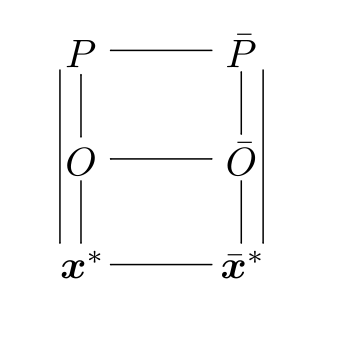
\includegraphics[width=0.2\columnwidth]{../ch4/figures/map}
\caption[Relationships between the original and scaled problems]{Relationships between the optimization formulations, optimality conditions, and optimal solutions for both the original and scaled problems. \label{fig:ch4:map}}
\end{figure}

% new paragraph
The following section will use the theory in this section to illustrate scaling in DO with some motivating examples.

%----------------------------------------------------------------
\section{Motivating Examples}
In this section, a number of examples of scaling in DO are presented. Some examples have direct application to existing design problems while others provide a more conceptual illustration. The examples in this section and the many uses described in Sec.~\ref{sec:ch4:uses} provide a strong foundation for using scaling in novel DO design problems. 

\subsection{Example 1: Simple SASA Problem\label{sec:ch4:sasa}}

This first example was developed to better understand the observed trends from an existing design study (for full details see Chapter~\ref{ch:7}).
The co-design study focused on developing a novel \glsfoo[noindex]{SASA} system for spacecraft pointing control and jitter reduction \cite{Chilan2017a}.
In this system, distributed piezoelectric actuators were used to strain the solar arrays, causing reactive forces that could be used to control the bus (spacecraft body) with higher precision, higher bandwidth, and reduced vibrations.

% new paragraph
The observed trend was an optimal constant ratio between the natural period of the first mode, \gls{firstperiod}, and time allotted for performing the maneuver, $t_f$ (which is visualized in Fig.~10 of Ref.~\cite{Chilan2017a}).
There was much discussion on why this ratio seemed to be constant and if there was any significance to the value of this optimal ratio (approximately $T_1/t_f = 4.41$).
To help provide some insight into these questions, a much simpler, but still representative, design problem was proposed.
In Fig.~\ref{fig:ch4:sasa_schematic}, both the original and simplified SASA systems are visualized. The simplified system modeled many of the fundamental phenomena present in the original high-fidelity system using a small number of lumped parameters.

\begin{figure}[t]
\centering
\includegraphics[width=0.6\textwidth]{../ch4/figures/sasa_schematic}
\caption[Illustrations of original and simplified strain-actuated solar array systems]{Illustrations of original and simplified strain-actuated solar array systems in Sec.~\ref{sec:ch4:sasa}. \label{fig:ch4:sasa_schematic}}
\end{figure}

The problem formulation for the simplified system is:
\begin{subequations}
\label{eq:ch4:sasa_prob_1}
\begin{align}
\min_{k,u(t)} \quad & - \theta(t_f) \\
\text{subject to:} \quad & J\ddot{\theta}(t) + k \theta(t) = u(t) \label{eq:ch4:diff_eq} \\
& \theta(0) = \dot{\theta}(0) = 0 \\
& \dot{\theta}(t_f) = 0 \\
& \abs{u(t)} \leq u_{\max}
\end{align}
\end{subequations}

\noindent where \gls{angle} is the relative displacement of the bus, $J$ is related to the inertia ratio between the solar arrays and bus, $u$ is an open-loop control moment applied to the solar array and is bounded by $u_{\glsfirst{max}}$, and \gls{spring} is the stiffness in the solar array.
The boundary constraints enforce the system to start at rest with zero energy and end at rest.
The optimization variables are both $k$ and $u(t)$.
Scaling can be applied to help analyze this DO problem.

\subsubsection{Standard Form}

First, we write the original DO problem in Eqn.~(\ref{eq:ch4:sasa_prob_1}) the standard form:
\begin{subequations}
\label{eq:ch4:sasa_prob_2}
\begin{align}
\min_{k,u(t)} \quad & - \xi_1(t_f) \\
\text{subject to:} \quad & \dot{\bm{\xi}} = \begin{bmatrix} 0 & 1 \\ -k/J & 0 \end{bmatrix} \bm{\xi} + \begin{bmatrix} 0 \\ 1/J \end{bmatrix} u \\
& \textcolor{light-gray}{\phi_1 := }\ \xi_1(0) = 0, \quad \textcolor{light-gray}{\phi_2 := }\  \xi_2(0) = 0 \\
& \textcolor{light-gray}{\phi_3 := }\  \xi_2(t_f) = 0 \\ 
& \textcolor{light-gray}{C_1 := }\  u - u_{\max} \leq 0, \quad \textcolor{light-gray}{C_2 := }\ -u - u_{\max} \leq 0 \\
\text{where:} \quad & \xi_1 = \theta, \quad \xi_2 = \dot{\theta}
\end{align}
\end{subequations}

\noindent The Hamiltonian is then:
\begin{align}
H = \lambda_1 \xi_2 + \lambda_2 \left( -\frac{k}{J} \xi_1 + \frac{u}{J} \right) + \mu_1 \left( u - u_{\max} \right) + \mu_2 \left( -u - u_{\max} \right)
\end{align}

\noindent Now using the conditions in Eqn.~(\ref{eq:ch3:opt_cond_sim}), the additional conditions for optimality are:
\begingroup
\allowdisplaybreaks
\begin{subequations}
\label{eq:ch4:sasa_cond_1}
\begin{gather}
\dot{\lambda}_1 = \frac{k}{J} \lambda_2, \quad \dot{\lambda}_2 = -\lambda_1  \\
0 = \frac{\lambda_2}{J} + \mu_1 - \mu_2 \\
0 = {\mu}_1 \left( u - u_{\max} \right), \ {\mu}_1 \geq 0, \quad 0 = {\mu}_2 \left( -u - u_{\max} \right), \ {\mu}_2 \geq 0 \\
0 = \nu_1 \xi_1(0), \ \nu_1 \neq 0, \quad 0 = \nu_2 \xi_2(0), \ \nu_2 \neq 0    \\
0 = \nu_3 \xi_2(t_f), \ \nu_3 \neq 0 \\
0 = \lambda_1(0) - 1 + \nu_1, \quad 0 = \lambda_2(0) + \nu_2 \\
0 = \lambda_1(t_f), \quad 0 = \lambda_2(t_f) - \nu_3 \\
0 = \int_0^{t_f} \lambda_2 \frac{\xi_1}{J} dt
\end{gather}
\end{subequations}%
\endgroup

\subsubsection{Scaled Form}

Consider the following change of variables based on linear scaling described in Sec.~\ref{sec:ch4:basics}:
\begin{gather}
t = \alpha_t \bar{t}, \quad u(t) = \alpha_{u} \bar{u}(t), \quad \theta(t) = \alpha_{\theta} \bar{\theta}(t)
\end{gather}

\noindent Next, the differential equation in Eqn.~(\ref{eq:ch4:diff_eq}) is parameterized as:
\begin{align}
J \frac{\alpha_{\theta}}{\alpha_t^2} \frac{d^2}{d\bar{t}^2}{\bar{\theta}} + k \alpha_{\theta}  \bar{\theta} = \alpha_u \bar{u}
\Rightarrow
\frac{d^2}{d\bar{t}^2}{\bar{\theta}} := {\bar{\theta}}''\gls{altderiv} = -k \frac{\alpha_t^2}{J} \bar{\theta} +  \frac{\alpha_u \alpha_t^2}{J \alpha_{\theta}} \bar{u}
\end{align}

\noindent The three parameters in the problem are $\{J, u_{\max}, t_f \}$.
There are three scaling constants to choose.
The following points are considered when deciding how to scale the problem based on some previous intuition:
\begin{enumerate}[label=$\bullet$, widest=$\bullet$, nosep]
\item Since all initial and final state conditions are zero, we should not start with $\alpha_\theta$
\item The time horizon should be fixed, i.e.,~independent of $t_f$
\item The magnitude of the control force should be unity to remove dependence on $u_{\max}$
\item It is fine to have $k$ multiplied by some constants since $k$ is an optimization variable and is not directly constrained
\item The natural period of this second-order system is $T = 2\pi \sqrt{{J}/{k}}$
\end{enumerate}

\noindent With these considerations, we select the values of the scaling parameters as:
\begin{align}
\alpha_t = \frac{t_f}{2\pi}, \quad \alpha_u = u_{\max}, \quad \alpha_\theta = \frac{u_{\max} t_f^2}{4 \pi^2 J} 
\end{align}

\noindent Note that the horizon is now fixed between $0$ and $2\pi$. Therefore, the scaled optimization problem is:
\begin{subequations}
\label{eq:ch4:sasa_prob_3}
\begin{align}
\min_{k, \bar{u}(\bar{t})} \quad & - \frac{u_{\max} t_f^2}{4 \pi^2 J}  \bar{\theta}(2\pi) \\
\text{subject to:} \quad & \bar{\theta}''  = - \frac{k t_f^2}{4 \pi^2 J} \bar{\theta} + \bar{u} \\
& \bar{\theta}(0) = \bar{\theta}'(0) = 0 \\
& \bar{\theta}'(2\pi) = 0 \\
& \abs{\bar{u}(\bar{t})} \leq 1
\end{align}
\end{subequations}

\noindent The scaled problem has two dimensionless quantities:
\begin{align}
\bar{\rho}_1 = \frac{k t_f^2}{4 \pi^2 J} \equiv \frac{t_f^2}{T^2}, \quad \bar{\rho}_2 = \frac{u_{\max} t_f^2}{4 \pi^2 J}
\end{align}

\noindent First, we have $\sqrt{\bar{\rho}_1} = t_f/T$, the exact ratio we are investigating.
We also have $\bar{\rho}_1$ as the only part of the formulation that depends on $k$ and since there are no constraints on $k$, we are effectively designing the quantity $\bar{\rho}_1$ directly.
Second, $\bar{\rho}_2$ is a positive constant linear factor in the objective function, so it will not affect the nature of the solutions \cite{Boyd2009a}, and it can be removed temporarily from the scaled formulation.
Therefore, the formulation is equivalent to the following DO problem in the standard form:
\begingroup
\allowdisplaybreaks
\begin{subequations}
\label{eq:ch4:sasa_prob_4}
\begin{align}
\min_{\bar{\rho}_1, \bar{u}(\bar{t})} \quad & - \mybar{\xi}_1(2\pi) \\
\text{subject to:} \quad & \dot{\mybar{\bm{\xi}}} = \begin{bmatrix} 0 & 1 \\ -\bar{\rho}_1 & 0 \end{bmatrix} \mybar{\bm{\xi}} + \begin{bmatrix} 0 \\ 1 \end{bmatrix} \bar{u} \\
& \textcolor{light-gray}{\phi_1 := }\ \mybar{\xi}_1(0) = 0, \quad \textcolor{light-gray}{\phi_2 := }\  \mybar{\xi}_2(0) = 0 \\
& \textcolor{light-gray}{\phi_3 := }\  \mybar{\xi}_2(2\pi) = 0 \\ 
& \textcolor{light-gray}{C_1 := }\  \bar{u} - 1 \leq 0, \quad \textcolor{light-gray}{C_2 := }\ -\bar{u} - 1 \leq 0 
\end{align}
\end{subequations}%
\endgroup

\noindent The dependence on the parameters $\bm{\rho} = \{J, u_{\max}, t_f \}$ has been removed completely; therefore, finding the single solution, $\bar{\bm{x}}^*$, to this scaled formulation will give all solutions for any valid $\bm{\rho}$!
We have also derived relationships to indicate how different values for these parameters directly affect the solution, i.e.,~the function $S$. 

\subsubsection{Equivalence of the Optimality Conditions}

It is still illustrative to show that there is a linear mapping between the $O$ and $\bar{O}$ for Probs.~(\ref{eq:ch4:sasa_prob_2}) and (\ref{eq:ch4:sasa_prob_4}).
The Hamiltonian for the scaled problem is:
\begin{align}
\mybar{H} = \mybar{\lambda}_1 \mybar{\xi}_2 + \mybar{\lambda}_2 \left( -\bar{\rho}_1 \mybar{\xi}_1 + \bar{u} \right) + \mybar{\mu}_1 \left( \bar{u} - 1 \right) + \mybar{\mu}_2 \left( -\bar{u} - 1 \right)
\end{align}

\noindent We expect some scaling of the multipliers between the two problems so we will define a scaling rule for each:
\begin{gather}
\begin{gathered}
\lambda_1 = \alpha_{\lambda_1} \mybar{\lambda}_1, \quad \lambda_2 = \alpha_{\lambda_2} \mybar{\lambda}_2, \quad \mu_1 = \alpha_{\mu_1} \mybar{\mu}_1, \quad \mu_2 = \alpha_{\mu_2} \mybar{\mu}_2 \\
\nu_1 = \alpha_{\nu_1} \mybar{\nu}_1, \quad \nu_2 = \alpha_{\nu_2} \mybar{\nu}_2, \quad \nu_3 = \alpha_{\nu_3} \mybar{\nu}_3
\end{gathered}
\end{gather}

\noindent To determine the proper values of the scaling constants, we need to substitute the change of variables into the optimality conditions in Eqn.~(\ref{eq:ch4:sasa_cond_1}):
\begingroup
\allowdisplaybreaks
\begin{subequations}
\label{eq:ch4:sasa_cond_2}
\begin{gather}
\frac{\alpha_{\lambda_1}}{\alpha_t} \dot{\mybar{\lambda}}_1 = \frac{k}{J} \alpha_{\lambda_2} \mybar{\lambda}_2, \quad \frac{\alpha_{\lambda_2}}{\alpha_t} \dot{\mybar{\lambda}}_2 = -\alpha_{\lambda_1} \mybar{\lambda}_1  \\
0 = \alpha_{\lambda_2} \frac{\mybar{\lambda}_2}{J} + \alpha_{\mu_1} \mybar{\mu}_1 - \alpha_{\mu_2} \mybar{\mu}_2 \\
0 = \alpha_{\mu_1} \mybar{\mu}_1 \left( \alpha_u \bar{u} - u_{\max} \right), \ \alpha_{\mu_1} \mybar{\mu}_1 \geq 0 \\
 0 =  \alpha_{\mu_2}  \mybar{\mu}_2 \left( -\alpha_u \bar{u} - u_{\max} \right), \ \alpha_{\mu_2} \mybar{\mu}_2 \geq 0 \\
0 = \alpha_{\nu_1} \mybar{\nu}_1 \alpha_\theta \mybar{\xi}_1(0), \ \alpha_{\nu_1} \mybar{\nu}_1 \neq 0 \\
0 = \alpha_{\nu_2} \mybar{\nu}_2 \frac{\alpha_\theta}{\alpha_t} \mybar{\xi}_2(0), \ \alpha_{\nu_2} \mybar{\nu}_2 \neq 0    \\
0 = \alpha_{\nu_3} \mybar{\nu}_3 \frac{\alpha_\theta}{\alpha_t} \mybar{\xi}_2(2\pi), \ \alpha_{\nu_3} \mybar{\nu}_3 \neq 0 \\
0 = \alpha_{\lambda_1} \mybar{\lambda}_1(0) - 1 + \alpha_{\nu_1} \mybar{\nu}_1, \quad 0 = \alpha_{\lambda_2} \mybar{\lambda}_2(0) + \alpha_{\nu_2} \mybar{\nu}_2 \\
0 = \alpha_{\lambda_1} \mybar{\lambda}_1(2\pi), \quad 0 = \alpha_{\lambda_2} \mybar{\lambda}_2(2\pi) - \alpha_{\nu_3} \mybar{\nu}_3 \\
0 = \alpha_t \int_0^{2\pi} \alpha_{\lambda_2}  \mybar{\lambda}_2 \frac{\alpha_\theta \mybar{\xi}_1}{J} d\tau
\end{gather}
\end{subequations}%
\endgroup

\noindent With the substitution applied, Eqn.~(\ref{eq:ch4:sasa_cond_2}) above should match the optimality conditions for Prob.~(\ref{eq:ch4:sasa_prob_4}) exactly.
This is accomplished with the following relationships:
\begin{align}
\alpha_{\lambda_1} = \alpha_{\nu_1}= 1, \quad \alpha_{\lambda_2} = \alpha_{\nu_2} = \alpha_{\nu_3} = J \alpha_{\mu_2} = J \alpha_{\mu_2} = \alpha_t
\end{align}

\noindent Thus, a simple linear map exists between the optimality conditions between the original and scaled forms.
The two Hamiltonians are related by\footnote{Using the objective $-\bar{\rho}_2 \bar{\theta}(2\pi)$, the relationship is $H = \alpha_\theta^2 \alpha_t \bar{H}$ with all multipliers containing an additional $\alpha_\theta$ term.}:
\begin{align}
H = \alpha_\theta \alpha_t \bar{H}
\end{align}

\subsubsection{Bounded Period}

An additional inequality was necessary to explain further the observed results from the original study.
This constraint was in the form of a bound on the period:
\begin{align}
T = \frac{t_f}{\sqrt{\bar{\rho}_1}} \leq T_{\max}
\end{align}

\noindent which can be written as:
\begin{align}
\label{eq:ch4:period_con}
\frac{t_f^2}{T_{\max}^2} - \bar{\rho}_1 := \bar{\rho}_3 - \bar{\rho}_1 \leq 0
\end{align}

\noindent where $\bar{\rho}_3$ is an additional dimensionless parameter.
We can denote $\bar{\rho}_1^{\glsfoo[noindex]{candidate}}$ as the optimal value for $\bar{\rho}_1$ without the additional constraint in Eqn.~(\ref{eq:ch4:period_con}).
If $\bar{\rho}_3 < \bar{\rho}_1^\dagger$, then the constraint is inactive, and the previous solution is valid.
However, if $\bar{\rho}_3 \geq \bar{\rho}_1^\dagger$, then the constraint is active and we would need to find solutions for every required value of $\bar{\rho}_3$ since the form of the optimal control will vary for each value of $\bar{\rho}_3$.
In this problem, the control remains bang-bang in nature but the number of switches increases and the switching locations vary (see Fig.~\ref{fig:ch4:sasa_control}).

\subsubsection{Solution}

\begin{figure}
\centering
\begin{subfigure}[b]{0.5\columnwidth}
    \centering
    % \includegraphics[width=\textwidth]{../ch4/figures/sasa_position}
    \includegraphics[width=\textwidth]{../ch4/figures/TP3_position}
    \caption{$\theta(t)$ and $\bar{\theta}(\bar{t})$.}
\end{subfigure}%
\begin{subfigure}[b]{0.5\columnwidth}
    \centering
    % \includegraphics[width=\textwidth]{../ch4/figures/sasa_control}
    \includegraphics[width=\textwidth]{../ch4/figures/TP3_control}
    \caption{$u(t)$ and $\bar{u}(\bar{t})$.\label{fig:ch4:sasa_control}}
\end{subfigure}
\caption[Scaled and unscaled solutions for the simple SASA problem]{Scaled and unscaled solutions for the simple SASA problem with $u_{\max} = 0.5$, $t_f = 3$, $J = 3$.\label{fig:ch4:sasa_plots}}
\end{figure}


With the optimization problem, optimality conditions, and optimal solutions thoroughly characterized, we can compare this simple SASA problem to the original design study in Ref.~\cite{Chilan2017a}. Both the scaled and unscaled solutions for the simple SASA problem without the additional bound on the period being active are shown in Fig.~\ref{fig:ch4:sasa_plots}.
There are a number of similarities between the trajectories in Ref.~\cite{Chilan2017a} and in Fig.~\ref{fig:ch4:sasa_plots}, including the bang-bang nature of the control when the period constraint is not active, and the general shape of the bus angle trajectories.

% new pargraph
The primary comparison is Fig.~\ref{fig:ch4:sasa_comparison}, which includes the results from Fig.~10 of Ref.~\cite{Chilan2017a}.
The figure plots the natural period of the first mode vs. $t_f$.
There is an observed linear trend until a period limit seems to be reached.
This is present for both design representations used: \glsfoo[noindex]{PLS} and \glsfoo[noindex]{VL}.
Both of these representations can change the structural properties of the solar array.
Although it is tough to see in the figure, there are coinciding data points at $t_f=0.12$ s for both cases indicating that there is a similar optimal value for $T_1$ (and ratio).

\begin{figure}
\centering
\includegraphics[width=0.6\textwidth]{../ch4/figures/sasa_comparison}
\caption[Natural period vs.~$t_f$ for the simple SASA and original design study]{Natural period vs.~$t_f$ results for the simple SASA problem and original design study in Chapter~\ref{ch:7}.\label{fig:ch4:sasa_comparison}}
\end{figure}

% new paragraph
Observing Fig.~\ref{fig:ch4:sasa_comparison}, there is a direct parallel between the data points and the simple SASA problem.
For the scaled problem, $\bar{\rho}_1^\dagger = 0.0866$ while the results from Ref.~\cite{Chilan2017a} indicate $\bar{\rho}_1$ should be approximately $0.0513$.
The difference may be attributed to the representation and constraints in the original design study.
Initial discussions of the results tried to pin the ratio $t_f/T_1$ to $1/4$ due to the periodic resonance of a simple beam.
However, the simple SASA problem suggests that this ratio is simply an arbitrary constant dependent on the interaction between the bang-bang controller and dynamics.
Continuing with the comparisons, the $T_{\max}$ bound seems to equal about $2.19$ s for the PLS case and $0.69$ s for the VL case.
If the physical-system constraints could be lifted, we have a reasonable prediction for how $T_1$ should vary.

% new paragraph
This example illustrated how scaling can be utilized effectively to obtain insights in a design study.

\subsection{Example 2: Co-Design Transfer Problem \label{sec:ch4:transfer}}

In this example, we will use scaling to transform a co-design problem into a form with a known solution\footnote{This problem was also used in Sec.~\ref{sec:ch3:transfer}.}. Consider the following co-design problem:
\begin{subequations}
\label{eq:ch4:ex2_prob_1}
\begin{align}
\min_{k, u(t)}  \quad & \int_{0}^{t_f} u^2 dt \\
\text{subject to:} \quad & \ddot{y} = - k y + u \\
& y(0) = y_0, \ \dot{y}(0) = v_0, \ y(t_f) = 0, \ \dot{y}(t_f) = 0
\end{align}
\end{subequations}

\noindent where $k$ is the time-independent, physical-system design variable and $u(t)$ is the open-loop control design variable.
Through scaling, we can transform Prob.~(\ref{eq:ch4:ex2_prob_1}) above into the problem in Ref.~\cite[pp.~166--167]{Bryson1975a}. 
To accomplish this, consider the following change of variables:
\begin{gather}
\label{eq:ch4:ex2_rules}
t = \alpha_t \bar{t}, \quad u = \alpha_u \bar{u}
\end{gather}

\begin{figure*}[t]
\centering
% \includegraphics[options]{name}

\begin{subfigure}[b]{0.5\textwidth}
    \centering
    \includegraphics[width=\textwidth]{../ch4/figures/transfer_psi}
    \caption{Objective function values.}
\end{subfigure}

\begin{subfigure}[b]{0.4\textwidth}
    \centering
    \includegraphics[width=\textwidth]{../ch4/figures/transfer_u}
    \caption{$u^*(t,k)$ for various values of $k$.}
\end{subfigure}%
\begin{subfigure}[b]{0.4\textwidth}
    \centering
    \includegraphics[width=\textwidth]{../ch4/figures/transfer_x}
    \caption{$y^*(t,k)$ for various values of $k$.}
\end{subfigure}

\caption[Co-design transfer problem]{Co-design transfer problem with $t_f = 1$, $x_0 = 1$, and $v_0 = 2$ (with $k^* = 6.924$).\label{fig:ch4:transfer_solution}}
\end{figure*}

\noindent We choose the following values for the scaling constants:
\begin{gather}
\alpha_t = \frac{1}{\sqrt{k}}, \quad \alpha_u = k
\end{gather}

\noindent where $k>0$. The case for $k=0$ needs to be handled separately.
Substituting in these scaling laws results in the following problem formulation:
\begin{subequations}
\label{eq:ch4:ex2_prob_2}
\begin{align}
\min_{k, \bar{u}(\bar{t})} \quad &  k^{3/2} \int_{0}^{\bar{t}_f} \bar{u}^2 d\bar{t} \\
\text{subject to:} \quad & y'' = - y + \bar{u} \\
& y(0) = y_0, \quad y'(0) = \bar{v}_0 \\ 
& y(\bar{t}_f) = 0, \quad y'(\bar{t}_f) = 0 \\
\text{where:} \quad & \bar{t}_f = \sqrt{k} t_f, \bar{v}_0 = v_0/\sqrt{k}
\end{align}
\end{subequations}

The solution to Prob.~(\ref{eq:ch4:ex2_prob_2}) above is readily available in Ref.~\cite{Bryson1975a}. Using this result and applying the scaling rules in Eqn.~(\ref{eq:ch4:ex2_rules}), we obtain the following solution for $u(t)$ as a function of $k$:
\begin{align}
\label{eq:ch4:ex2_usol}
\begin{aligned}
u^*(t,k) &= - \frac{2k}{k t_f^2 - \sin^2(\sqrt{k} t_f)} \left( c_1(t,k) x_0 + c_2(t,k) \frac{v_0}{\sqrt{k}} \right) \\
c_1(t,k)  &= \sin\left( \sqrt{k}(t_f - t) \right)\sin\left(\sqrt{k}t_f\right) - \sqrt{k} t_f \sin \left(\sqrt{k}t \right) \\
c_2(t,k)  &= - \cos\left(\sqrt{k}(t_f-t)\right) \sin\left(\sqrt{k}t_f\right) + \sqrt{k} t_f \cos\left(\sqrt{k}t\right)
\end{aligned}
\end{align}

\noindent For certain problem parameter values, the solution for various values of $k$ is shown in Fig.~\ref{fig:ch4:transfer_solution}. 
The original objective function can now be computed analytically with Eqn.~(\ref{eq:ch4:ex2_usol}).
With this closed-form expression for the objective function, an optimality condition for $k$ can be derived.
This property makes this problem quite suitable for investigations between nested and simultaneous co-design methods and can be used to illustrate a number of concepts found in many co-design problems (such as open-loop control, multiple optima, degenerate plant designs, and a system-level objective function) \cite{Herber2017b}.

% new paragraph
For many DO problems, obtaining a closed-form solution for a portion of the design variables may not be possible. 
Observing different (but equivalent) forms of the same design optimization formulation can facilitate a better understanding of the design problem.
In this example, we see that for larger values of $k$, the scaled problem has a larger time horizon but smaller initial velocity. 

% new paragraph
In addition, these different forms may be more suitable computation depending on the parameter values.
In this example using the original Prob.~(\ref{eq:ch4:ex2_prob_1}) formulation, large values of $k$ would result in highly oscillatory solutions.
With the time-horizon fixed, large discretization errors would start appearing in the solutions with a fixed number of time points if a DT solution method was utilized. This helps motivate the final example.

\subsection{Example 3: Direct Transcription Discretization \label{sec:example3}}

DT is a popular solution method for solving DO problems and is described in more detail in Chapter~\ref{ch:5} \cite{Biegler2010a, Betts2010a, Allison2014b,Allison2014a}.
In this approach, the dynamics are approximated with a large number of equality constraints, termed defect constraints.
Equality constraints in a NLP are typically of the form $h(\bm{x}) = 0$. However, most numerical algorithms implement this constraint type as two inequality constraints as:
\begin{align}
\label{eq:ch4:ineq_error}
- \epsilon \leq h(x) \leq \epsilon
\end{align}

\noindent where \gls{epsilon} is a small tolerance number (e.g.,~the default tolerance in \textsc{Matlab}'s \texttt{fmincon} function is $\epsilon = 10^{-6}$ \cite{matlab-fmincon}).
In this example, we will demonstrate how the absolute magnitudes of the state variables can greatly degrade direct transcription approximations.

Consider the simple scalar system:
\begin{align}
\label{eq:ch4:dt_original}
\dot{y} = a y, \quad y(0) = y_0
\end{align}

\noindent where the solution to this set of DAEs is $\hat{y}(t) = y_0 e^{at}$. We can introduce a change of variables as:
\begin{align*}
t = \alpha_t \bar{t}, \quad y = \alpha_y \bar{y}
\end{align*}

\noindent where the scaling constants are $\alpha_t = \abs{a}$ and $\alpha_y = y_0$, resulting in the following scaled system:
\begin{align}
\bar{y}' = \bar{y}, \quad \bar{y}(0) = 1
\end{align}

\noindent We can now see how the relative error is influenced by the different systems.

% new paragraph
A basic single-step DT method is the trapezoidal rule and the defect constraint that ensures accurate dynamics has the following form for a scalar ODE:
\begin{align}
\label{eq:ch4:defect}
0 &= y_k - y_{k-1} - \frac{\Delta_k}{2}\Big( f(t_{k-1}, y_{k-1}) + f(t_k, y_{k}) \Big)
\end{align}

\noindent where $y_k$ is the approximate value of $y(t)$ at $t_k$, $\glsfirst{stepsize}_k = t_k - t_{k-1}$ is the step-size parameter, and $f(t_k, y_{k})$ is the value of the derivative function at $t_k$.

We will consider the initial step, i.e.,~$k=1$. Then the DT constraint for Eqn.~(\ref{eq:ch4:dt_original}) is:
\begin{align}
0 &= y_1 - y_{0} - \frac{\Delta_1}{2} \left( a y_{0} + a y_1 \right)
\end{align}

Using the tolerances in Eqn.~(\ref{eq:ch4:ineq_error}), we can derive the minimum and maximum values for $y_1$ that still satisfy the constraint:
\begin{align}
\frac{\left(1+\Delta_1 a/2\right) y_0 - \epsilon}{\left(1-\Delta_1 a/2\right)} \leq y_1 \leq \frac{\left(1+\Delta_1 a/2\right) y_0 + \epsilon}{\left(1-\Delta_1 a/2\right)}
\end{align}

\noindent Alternatively, the bounds for $\bar{y}_1$ are:
\begin{align}
\frac{\left(1+\mathrm{sign}(a)\Delta_1/2\right) - \epsilon}{\left(1-\mathrm{sign}(a)\Delta_1/2\right)} \leq \bar{y}_1 \leq \frac{\left(1+\mathrm{sign}(a)\Delta_1/2\right) + \epsilon}{\left(1-\mathrm{sign}(a)\Delta_1/2\right)}
\end{align}

\noindent The relative error is defined as:
\begin{align}
\gls{relerror} = \frac{y_1 - \hat{y}_1}{\hat{y}_1} = \frac{y_1 - y_0 e^{a t_1}}{y_0 e^{a t_1}}, \quad \bar{e}_r = \frac{\bar{y}_1 - e^{\mathrm{sign}(a) t_1}}{ e^{\mathrm{sign}(a) t_1}}
\end{align}

Now, consider the following values for the problem and DT parameters: $y_0 = 10^{-6}$, $a = 2$, $\epsilon = 10^{-6}$, $\Delta_1 = 10^{-3}$. For these values, we have the following relative error bounds:
\begin{subequations}
\begin{gather}
-9.99 \times 10^{-1} \leq e_r \leq 9.99 \times 10^{-1} \\
-9.99 \times 10^{-7} \leq \bar{e}_r \leq 9.99 \times 10^{-7}
\end{gather}
\end{subequations}

\noindent We see that the $e_r$ is quite poor using the original system while $\bar{e}_r$ is right around the expected $\epsilon$ tolerance. Consider one more choice of parameters: $y_0 = 10^{3}$, $a = -1$, $\epsilon = 10^{-6}$, $\Delta_1 = 10^{-3}$ and error bounds: 
\begin{subequations}
\begin{gather}
-1.08 \times 10^{-9} \leq e_r \leq 9.13 \times 10^{-10} \\
-1.00 \times 10^{-6} \leq \bar{e}_r \leq 1.00 \times 10^{-6}
\end{gather}
\end{subequations}

\begin{figure}
\centering
\begin{subfigure}[b]{0.5\textwidth}
    \centering
    \includegraphics[width=\textwidth]{../ch4/figures/dt_errors_1}
    \caption{$y_0 = 10^{-6}$ and $a = 2$.\label{fig:ch4:dt_errors_1}}
\end{subfigure}%
\begin{subfigure}[b]{0.5\textwidth}
    \centering
    \includegraphics[width=\textwidth]{../ch4/figures/dt_errors_2}
    \caption{$y_0=10^2$ and $a=-1$.\label{fig:ch4:dt_errors_2}}
\end{subfigure}
\caption[Maximum absolute relative error vs. step size for defect constraints]{Maximum absolute relative error vs. step size for original and scaled defect constraints.\label{fig:ch4:dt_errors}}
\end{figure}


\noindent Now we see that the relative error bounds are tighter than $\epsilon$ which could lead to numerical issues. The scaled form, however, is still right around the $\epsilon$ tolerance. The maximum absolute relative error vs. step size is shown in Fig.~\ref{fig:ch4:dt_errors}. From these plots, we see that for a sufficiently small step size, the scaled system has error bounds near $\epsilon$.

Both of these parameter sets show the importance of scaling the dynamics to be near unity when using a DT implementation.
Since DT implementations use a large number of linked defect constraints, the errors can compound, potentially producing highly inaccurate results.
Additionally, scaling the time horizon provides a more uniform method for selecting $\Delta$ to achieve suitable accuracy without too many optimization variables (note that $\Delta_1=10^{-3}$ for $\bar{e}_r$ is quite good in both plots). Finally, scaling the states to be near unity is also produces computationally favorable matrices (Hessian/Jacobians) and finite differencing \cite{Rao2010a, Betts2010a}.

\section{Summary\label{sec:ch4:conclusion}}

In this chapter, we explored scaling in DO with a particular focus on how to leverage scaling in design optimization.
A review of the large amount of work around scaling was provided.
The necessary theory for scaling DO formulations was presented and a number of novel motivating examples were provided.
Scaling was shown to help facilitate finding accurate, generalizable, and intuitive information.

% new paragraph
At a basic level, scaling is simply the stretching, squeezing, and shifting of the problem elements such as the time continuum, design variables, constraints, and objective function. 
The unique structure of DO suggests that scaling can be utilized in novel ways to provide better analysis and formulations more favorable for different solution methods.
The mechanics of scaling are fairly straightforward but proper utilization of scaling is heavily reliant on the creativity and intuition of the designer.
This nebulous qualification is the primary limitation on the use of scaling. However, scaling is also limited by the scaling law chosen, the structure of the problem, and the number of free parameters.
Furthermore, scaling does not remove optimization; we still need to solve some form of the optimization problem.
Improper use of scaling can lead to incorrect solutions/insights or amplification of numerical issues rather than mitigation.

% new paragraph
Aiding the designer in constructing the appropriate scaled formulations needs compelling examples.
In the simple SASA problem, scaling was used to understand observed results from more complete, higher-fidelity design study. The simpler scaled optimization problem and dimensionless variables provided a number of insights. 
In the second example, the solution to a co-design problem was found by leveraging a scaled formulation with the known solution.
Observing different (but equivalent) forms of the same design optimization formulation can facilitate a better understanding of the design problem.
In the final example, the discretization error of one of the popular solution methods (namely direct transcription) for DO was explored. The scaled system showed much more favorable properties than the original.
Additional work is needed to develop general guidelines to aid in balancing the many uses of scaling.